\documentclass[letterpaper]{article}
\usepackage[submission]{aaai2027}
\usepackage{url}
\usepackage{graphicx}
\urlstyle{rm}
\def\UrlFont{\rm}
\usepackage{natbib}
\usepackage{caption}
\frenchspacing
\hyphenpenalty=10000
\exhyphenpenalty=10000
\emergencystretch=2em
\usepackage{amsmath,amssymb,booktabs,array}
\setcounter{secnumdepth}{2}
\pdfinfo{/TemplateVersion (2027.1)}
\title{Auditing Feature Populations and Label Selectivity in Brain MRI}
\author{Anonymous Authors}
\affiliations{}
\setlength{\textfloatsep}{14pt plus 2pt minus 4pt}
\begin{document}
\setlength{\parindent}{0pt}
\setlength{\parskip}{2pt}
\maketitle
\begin{abstract}
We compare how consistently sparse autoencoder (SAE) features select slices with the same label in brain tumour MRI. The answer depends on which features are included and how tumour area and slice position are taken into account. Across all eligible features, NCL leads SimCLR by 4.11 percentage points in raw purity. When both methods show eight features ($J=8$), NCL trails by $8.19$ points, with a conditional patient resampling envelope of $[-12.50,-1.25]$. The mean gap crosses zero between budgets of about 64 and 70 and reaches $+1.04$ points at $J=80$. The envelopes for larger budgets include zero. At $J=64$, ranking by training activity gives NCL purity 0.98 points below its own random subset average and gives SimCLR purity 3.25 points above its own average. The NCL lead is also unclear when we shuffle labels among slices with similar tumour area and position. SimCLR predicts tumour presence better from raw embeddings and full SAE codes, while NCL leads when the probes use 64 selected features. We also include a supervised reference. Our results show why comparisons should report which features were included, how many could be scored, what reference was used and which representation was tested for prediction. The results are exploratory because we reuse the validation patients used to choose checkpoints.
\end{abstract}

\section{Introduction}
The slices that activate an SAE feature most strongly can share a label because they show no tumour, have tumours of similar size or come from similar positions in the scan. A gallery of those slices can look convincing without identifying a medical concept. We study this problem in fluid attenuated inversion recovery (FLAIR) MRI, using one imaging channel and labels derived from expert segmentations. We compare two contrastive methods and a supervised reference. We ask how three choices affect the comparison: which features to score, which annotation context to account for and what to predict. Research on shortcut learning motivates this distinction between label agreement and the image evidence a model uses \cite{geirhos2020shortcut}.

Figure~\ref{fig:auditidea} summarizes the distinction between image context, feature population and the statistic being compared. A high average over one population need not persist at a fixed feature budget or relative to a context preserving reference.

We compare SimCLR \cite{chen2020simple} with existing nonnegative contrastive learning \cite{wang2024nonnegative}. NCL adds a terminal ReLU at the training projector; our SAE decomposes the signed \emph{backbone} CLS representation. The contribution is an empirical evaluation of these existing methods.

We make three contributions. First, we compare purity over a range of feature budgets, use random subsets as a reference and report bounds when some features cannot be scored. Second, we compare purity against labels shuffled within groups defined by tumour area and slice position. Third, we examine how purity relates to prediction from one feature at a time. This last comparison shares information with the shuffle reference and is descriptive. These procedures use existing statistics and reuse the original checkpoint selection cohort.

\begin{figure*}[t]
\centering
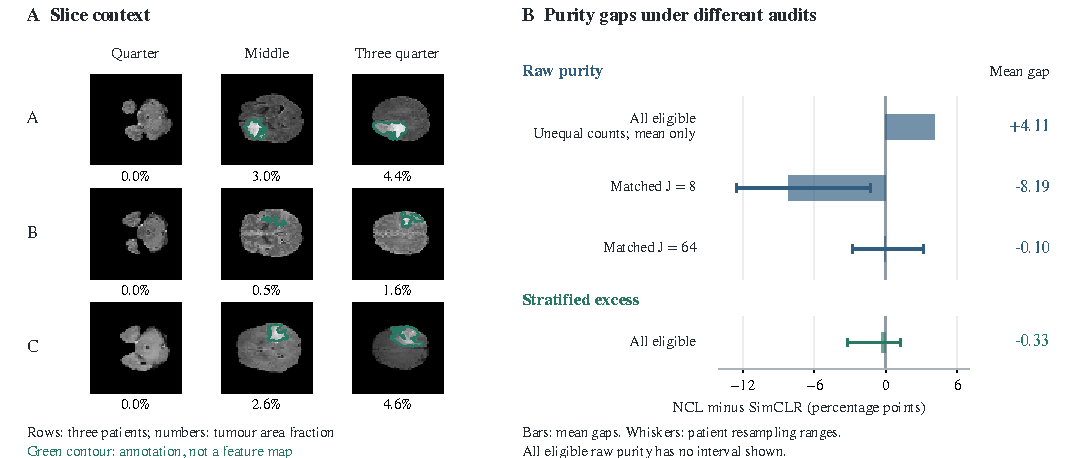
\includegraphics[width=\textwidth]{figures/audit_idea.pdf}
\caption{Nine FLAIR slices: rows are the first three validation patients; columns are quarter, middle and three quarter retained slice positions. Numbers give tumour area fractions; green contours are annotations. Bars show mean NCL minus SimCLR gaps; whiskers show conditional patient resampling ranges with missing support bounds (Section~\ref{sec:uncertainty}). The unequal population raw comparison shows its mean only.}
\label{fig:auditidea}
\end{figure*}

\section{Related Work and Scope}
\paragraph{The encoder comparison.}
SimCLR learns paired view contrastive representations \cite{chen2020simple}; NCL constrains the projector output to be nonnegative \cite{wang2024nonnegative}. Alignment and uniformity characterize contrastive geometry \cite{wang2020alignment}, while dimensional collapse motivates separating backbone and projector behavior \cite{jing2022dimensionalcollapse}. Our study audits these existing methods rather than proposing another encoder objective.

\paragraph{SAE feature evaluation.}
TopK SAEs impose an activation budget \cite{gao2024scaling}. SAEBench emphasizes multiple evaluation outcomes and Paulo and Belrose examine seed dependent feature recovery \cite{karvonen2025saebench,paulo2025differentfeatures}. Gated and JumpReLU SAEs change feature inference \cite{rajamanoharan2024gated,rajamanoharan2024jump}; shaping and geometry guided fitting offer other interventions \cite{delafrooznoroozi2026shaped,nerrise2026geosae}. We keep the native TopK recipe fixed and audit population, context and coverage rather than comparing these alternatives.

\paragraph{The interpretation target.}
Shortcut learning distinguishes label agreement from the evidence used by a model \cite{geirhos2020shortcut}. Concept based evaluations test alignment or sensitivity to specified concepts \cite{bau2017dissection,kim2018tcav}, while clinical critiques require validation beyond plausible explanations \cite{ghassemi2021falsehope}. Our outcome is coarse slice label selectivity, not clinical semantic validity. Appendix~\ref{app:relatedcontext} places this audit within broader representation and explanation research.

\section{Data and Representation Pipeline}
\subsection{Cohort and targets}
We use BraTS glioma MRI \cite{menze2014multimodal,baid2021brats,bakas2017advancing,bakas2017gbmdata,bakas2017lggdata}. The labelled BraTS 2023 GLI archive has 1,251 cases, grouped into 1,133 identities using transitive base GLI and shared BraTS 2017 to 2021 mapping IDs. The lexicographically smallest case represents each training group, not an assumed clinical baseline. Groups linked to the original BraTS 2020 validation/test patients are excluded from training; those patients retain their processed slices. The cohort contains 1,059 training groups (138,399 slices), 37 validation patients (4,761 slices) and 37 registered test patients (4,821 slices). Mapping groups and manifest patients are split disjoint; undocumented duplicates remain possible. No older training cohort or unlabelled challenge validation data are appended. The source audit retains identity mappings and lineage.

Data used in this publication were obtained as part of the Brain Tumor Segmentation (BraTS) Challenge project through Synapse ID: syn51156910. The stated Creative Commons Attribution NonCommercial 4.0 terms apply. Imaging data are not redistributed.

Each input is a normalized, single channel axial FLAIR slice resized to $128\times128$. The binary target is whether the slice contains tumour mask pixels. A separate dominant region label is the largest nonzero annotated region when tumour is present; label 0 is used only when no tumour is present. Thus the dominant label is not a spatial explanation target. In validation, class frequencies are 2,373 non tumour, 358 necrotic/core, 1,717 edema and 313 enhancing tumour slices. Edema is the largest tumour region class, but non tumour is the largest class overall.

\subsection{Encoder and training objective}
We use the vision transformer architecture \cite{dosovitskiy2021vit} at the Tiny model scale \cite{touvron2021deit}. Let $I_i$ denote an input and $h_i=f_\theta(I_i)\in\mathbb R^d$ its ViT Tiny CLS vector. We use $d=192$ and a projector $g_\psi:\mathbb R^d\to\mathbb R^q$, with $q=128$:
\begin{equation}
z_i=\begin{cases}g_\psi(h_i),&\text{SimCLR},\\
\operatorname{ReLU}(g_\psi(h_i)),&\text{NCL}.
\end{cases}\label{eq:projector}
\end{equation}
The backbone and projector are trained together on two augmented views of each slice. With batch size $B=64$, normalized outputs $\bar z_i=z_i/\max(\|z_i\|_2,\epsilon)$, paired view index $p(i)$ and temperature $\tau=0.5$, the contrastive loss is
\begin{equation}
\mathcal L_{\rm con}=-\frac{1}{2B}\sum_{i=1}^{2B}
\log\frac{\exp(\bar z_i^\top\bar z_{p(i)}/\tau)}
{\sum_{j\ne i}\exp(\bar z_i^\top\bar z_j/\tau)}.
\label{eq:contrastive}
\end{equation}
The encoder seeds are 10, 42 and 52, each trained for 50 epochs at learning rate $5\times10^{-4}$. Checkpoint selection used the validation objective; subsequent analyses reuse the same 37 validation patients and are therefore exploratory. Both contrastive methods use the same optimization budget and paired view augmentations. The supervised reference uses binary labels and its own augmentation regime. Encoders use AdamW with weight decay .01 and 16 pixel patches.

\begin{figure*}[t]
\centering
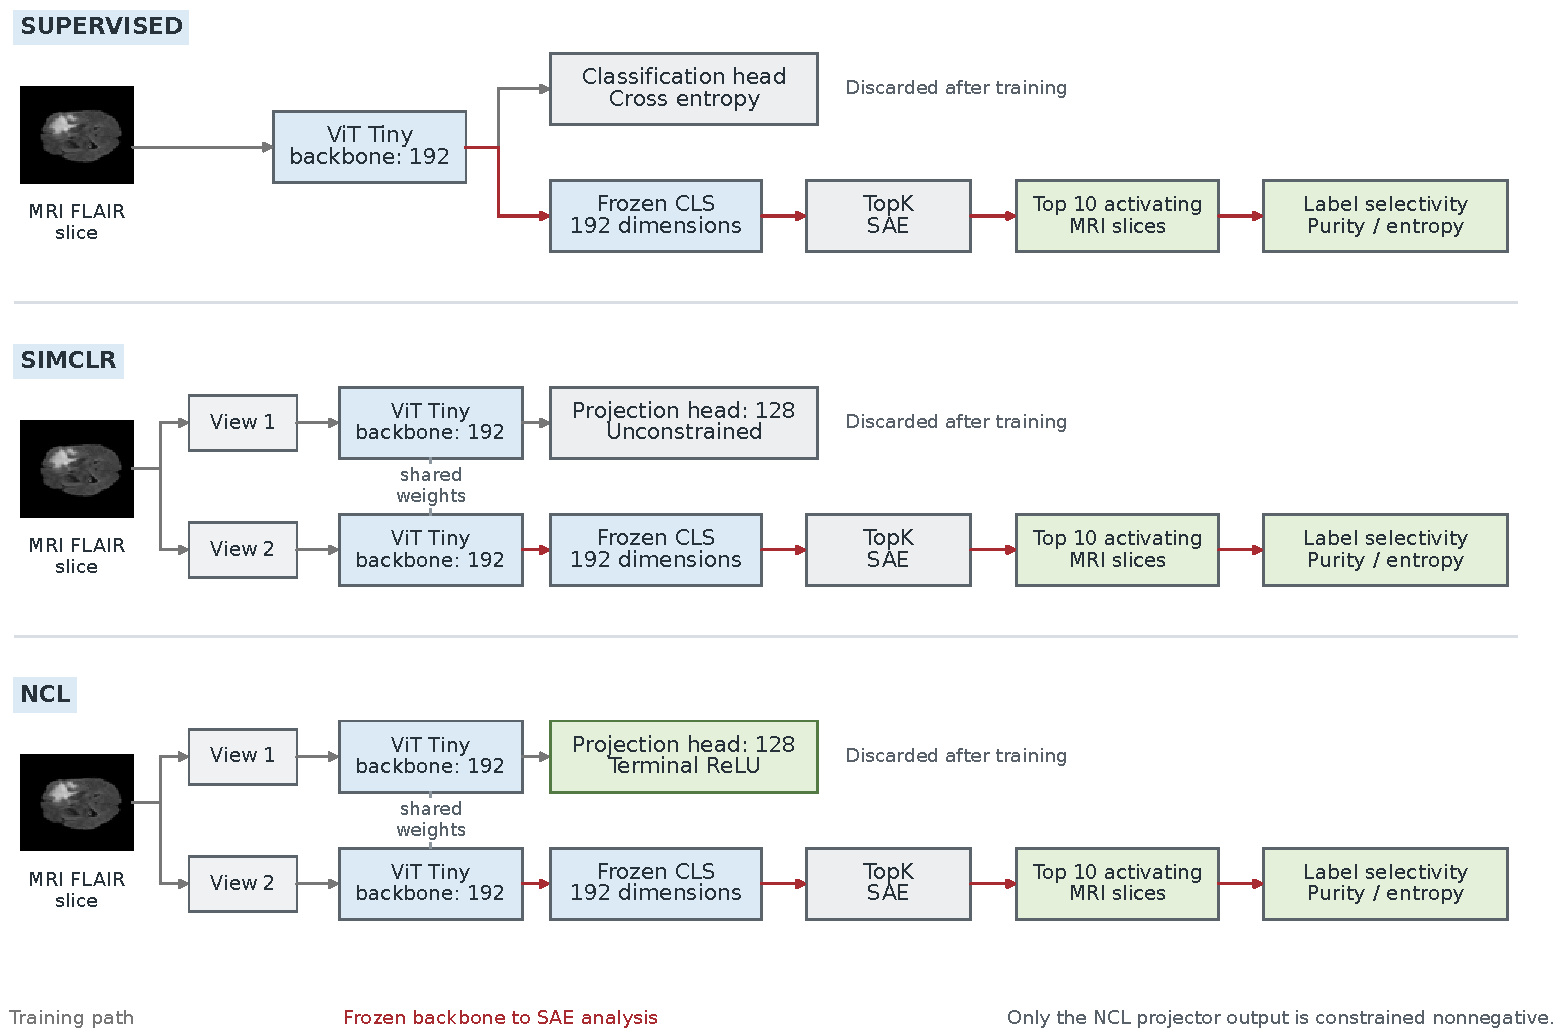
\includegraphics[width=\textwidth]{figures/pipeline.pdf}
\caption{Encoder training and frozen backbone analysis. Gray arrows show training paths; red arrows show the SAE audit. The paired views illustrate training with shared backbone weights; audit vectors are extracted separately from unaugmented slices using the frozen backbone. Training heads are discarded before SAE fitting. Only the NCL projector output is constrained nonnegative. Raw CLS and SAE code probes follow Section~\ref{sec:probes}.}
\label{fig:pipeline}
\end{figure*}

\subsection{Frozen backbone SAEs}
Figure~\ref{fig:pipeline} separates the training constraint from the evaluated object. After training, we discard the projector and compute the training mean $\mu_{\rm tr}$. Write $x_i=h_i-\mu_{\rm tr}$. For learned input bias $b_0$, encoder bias $b_e$ and matrices $W_e\in\mathbb R^{D\times d}$ and $W_d\in\mathbb R^{d\times D}$, the SAE is
\begin{align}
a_i&=\operatorname{TopK}\!\left(\operatorname{ReLU}
 (W_e(x_i-b_0)+b_e),K\right),\nonumber\\
\hat x_i&=W_da_i+b_0.\label{eq:sae}
\end{align}
TopK keeps at most $K$ positive activations per slice. We subtract the training mean and fit dictionaries with $D=1536=8d$ and $K=24$. We train each SAE for 30 epochs, using seeds 10, 42 and 52. Adam uses a learning rate of $5\times10^{-4}$, batches of 512 and gradient clipping at 1. We use the default PyTorch initialization, untied weights and no decoder normalization. We reuse the archived NCL and SimCLR dictionaries. We fit nine supervised SAEs to saved encoder vectors with the same recipe. In total, the audits use 27 dictionaries and require no encoder retraining. The supervised encoder uses a different target and different augmentations, so we include it as a reference.

\section{Audit Procedures}
Table~\ref{tab:procedures} summarizes the three questions. Settings were frozen before these additional computations, after prior validation inspection; code, input hashes and outputs are retained.

\begin{table}[t]
\centering\small
\begin{tabular}{@{}>{\raggedright\arraybackslash}p{.77in}>{\raggedright\arraybackslash}p{.97in}>{\raggedright\arraybackslash}p{1.03in}@{}}
\toprule
Procedure & Question answered & Key result\\\midrule
Budgets and random subsets & Does the displayed population change the ranking? & Mean rankings change; larger budget patient envelopes span zero.\\
Stratified null & Is purity unusual beyond area/position label mix? & NCL's positive lead is not retained.\\
Feature wise AUROC & How do purity and prediction relate? & Shared target structure limits interpretation.\\
\bottomrule
\end{tabular}
\caption{Audit procedures and their descriptive findings on the reused validation cohort.}
\label{tab:procedures}
\end{table}

\subsection{Label purity and feature populations}
Let $c_i\in\{0,1,2,4\}$ be the dominant region label and $a_{ij}\geq0$ the activation of feature $j$. A feature is scorable if its validation support $S_j=\sum_i\mathbf1[a_{ij}>0]$ is at least $M=10$. For the ten highest positive slices $U_j$, with sample order tie breaks,
\begin{equation}
 P_j=\max_c\frac1M\sum_{i\in U_j}\mathbf1[c_i=c].
\label{eq:purity}
\end{equation}
We average $P_j$ over the eligible set $\mathcal E=\{j:S_j\geq M\}$. Each dictionary can contribute a different set of features. The four labels tell us how consistent the top slices are, but do not show where in a slice a feature responds.

\subsection{Feature level predictive association}
We use each feature's activation as a score for tumour presence. Training AUROC sets the direction of the score: $s_j=1$ if training AUROC is at least $.5$ and $s_j=-1$ otherwise. We then compute validation AUROC as $A_j=\operatorname{AUROC}(y,s_ja_j)$, which measures how well the score ranks the two classes \cite{hanley1982auc}. We use Spearman correlation \cite{spearman1904association} to compare $A_j$ with purity for the same scorable features. A positive association is partly expected because both measures distinguish slices with and without tumour. Purity uses four labels and AUROC uses two. The analysis measures one feature at a time and leaves open how features work together or what happens if we remove one.

\subsection{Aggregate predictive probes}\label{sec:probes}
We train logistic regression to predict whether a slice contains tumour. The inputs are either raw frozen CLS vectors, all 1,536 SAE activations or a code with 64 selected features. All probes use L2 regularization with $C=1$, an intercept, the limited memory BFGS solver, a tolerance of $10^{-4}$ and at most 2,000 iterations. We use the same settings for all methods and no class weights. We standardize raw vectors with training means and standard deviations. For sparse codes we divide by the training standard deviations and let the intercept account for the mean. On validation we use a probability threshold of 0.5 and average the F1 scores for slices with and without tumour to get macro F1. We choose the 64 features from those eligible on validation, rank them by positive training activations and break ties by feature index. For SAE probes we average fits within each encoder before averaging across encoders. For raw probes we average across encoder seeds. These results describe slice predictions on the reused validation cohort.

\subsection{Stratified reference purity}
A global label shuffle preserves overall frequencies but not context within a feature's top examples. Our primary reference separates zero tumour area, divides positive mask area fraction into four quantile bins and crosses these with four axial index quantile bins. Cutpoints are fixed from validation covariates without optimizing feature purity. Let $B(i)$ denote the resulting cell. In each of $R=1000$ draws, labels are permuted only within the same cell:
\begin{equation}
 E_j=P_j-\frac1R\sum_{r=1}^{R}P_j\bigl(c^{(r)}\bigr),\quad
 c^{(r)}=\operatorname{Permute}(c\mid B).
\label{eq:stratified}
\end{equation}
We keep the same top slices for each feature and report $E_j$ alongside a global reference based on 1,000 shuffles. We also repeat the stratified analysis with three and five bins. The tumour masks define area, so the zero area group preserves tumour absence by design. This reference describes label concentration and requires annotations. It does not estimate a causal effect or provide a patient level permutation test. We record the bin edges, counts and label mix. As a check, an oracle that selects only slices without tumour has 100\% purity and zero excess. A second oracle selects ten slices with label 4 from a mixed stratum and retains 33.94 points of excess. These examples show that excess can detect concentration beyond the group label mix. Validating learned features or clinical meaning requires separate evidence.

\subsection{Budget curves and random subset references}
We select features in two ways. The first compares equally sized galleries using features that can be scored on validation. The second selects features from training data alone and checks how many can be scored on validation.

Both rules rank features by how often they activate in training. Ties are broken by feature index. We test every integer budget $J\geq8$ up to the number of eligible features in each dictionary. We compare methods at the same budget only when all nine dictionaries from each method can contribute. For NCL and SimCLR, this gives a common range of $8\leq J\leq87$. Outside that range, the curves show which features each method has available.

The training only selector freezes the first $J$ training used IDs. If only $n_J$ are scorable, report their conditional mean and the full budget bounds
\begin{equation}
 L_J=\frac{\sum_{j\in F_J\cap\mathcal E}P_j}{J},\qquad
 U_J=L_J+\frac{J-n_J}{J},
\label{eq:bounds}
\end{equation}
where $F_J$ is the frozen selected set. No unit is replaced. The difference bounds are $[L_{J,\mathrm{NCL}}-U_{J,\mathrm{SimCLR}},U_{J,\mathrm{NCL}}-L_{J,\mathrm{SimCLR}}]$. The unchanged training only $J=32$ NCL/SimCLR selection repeats the original result; it is not independent evidence.

For each selection rule, we shuffle the candidate features 1,000 times and take the first $J$ in each shuffle. This draws features without replacement and lets us use the same shuffles across budgets. For each fit, the draws give reference quantiles and show where the activity ranked mean falls. Random subsets test whether the ranking rule changes purity. Shuffling labels tests whether the top slices share labels more often than expected under the reference.

\subsection{Aggregation and uncertainty}\label{sec:uncertainty}
We bootstrap patients \cite{efron1979bootstrap}. For descriptive summaries and correlations, we first average SAE seeds within each encoder, then report the mean and standard deviation across three encoders. Random subset quantiles describe variation from feature selection. The patient bootstrap describes variation across patients for the fitted models.

For Figure~\ref{fig:budgetaudit}B, we draw 2,000 paired samples of 37 patients. We keep all slices from each sampled patient, including repeats. We hold the fitted models and selected features fixed and recompute top ten purity. Features that cannot be scored keep $[0,1]$ bounds. The shaded range runs from the 2.5th percentile of the lower gap bounds to the 97.5th percentile of the upper bounds. It applies at each budget separately and has no guaranteed coverage. We report a complete case interval only if 95\% of draws can score every selected feature. For Table~\ref{tab:context}, we draw 1,000 paired patient samples and recompute the top tens, AUROC and within group label shuffles (1,000 per draw). We keep the models, score directions and bin edges fixed but reapply the eligibility rule. These percentile ranges exclude uncertainty from training and analysis choices. Their coverage is not calibrated for top ten statistics.

\begin{figure*}[t]
\centering
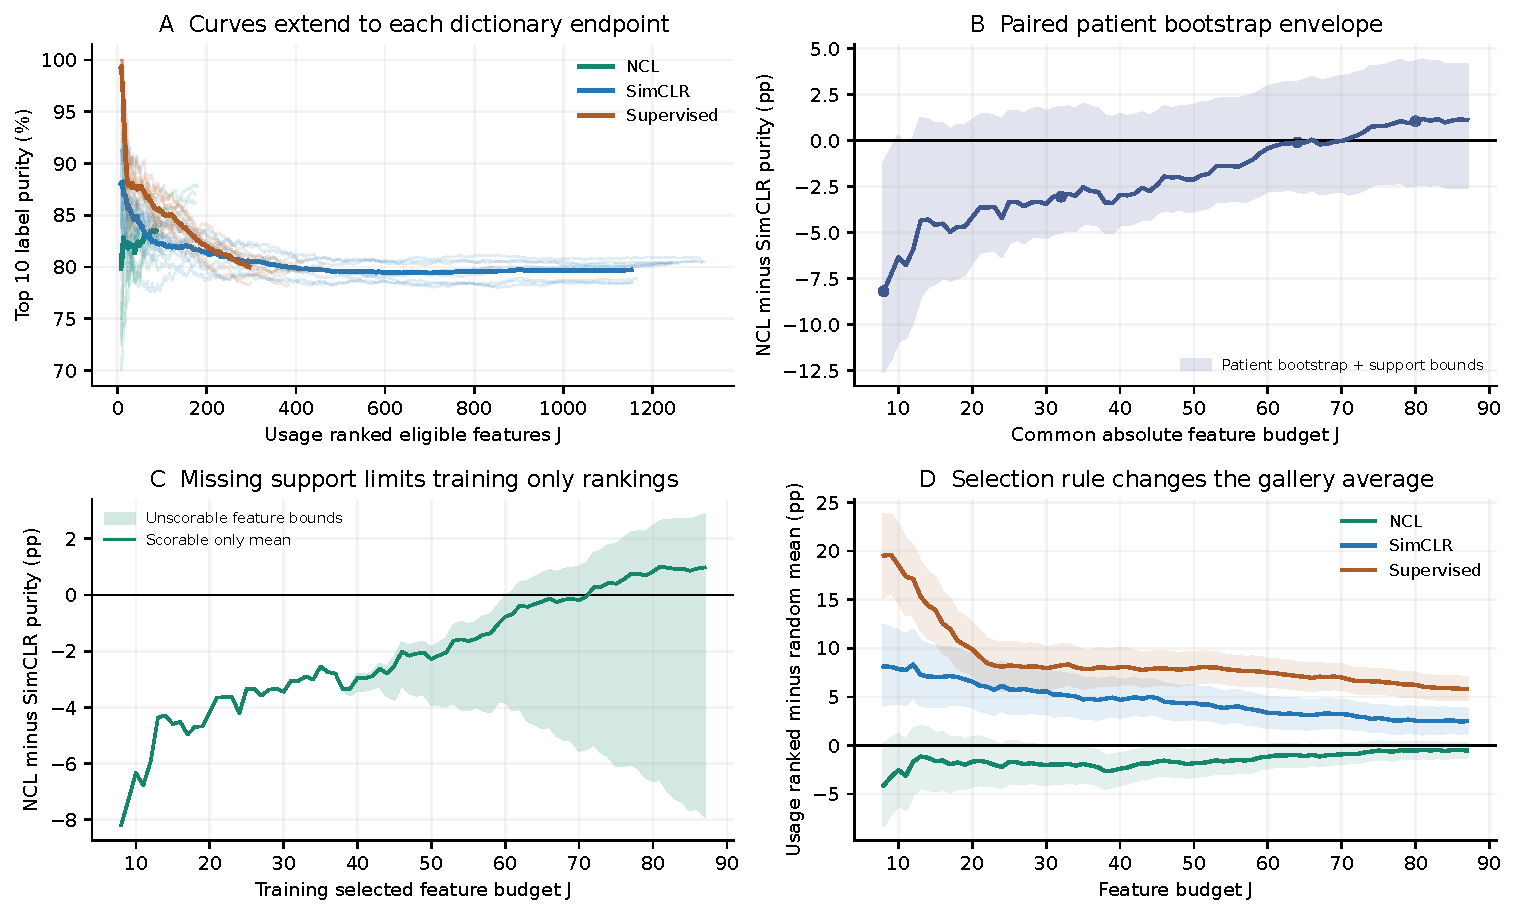
\includegraphics[width=\textwidth]{figures/feature_budget_audit.pdf}
\caption{Feature population audit. A: faint curves extend to eligible endpoints; thick curves retain all replications. B: equal $J$ gap with a pointwise 2,000 draw paired patient bootstrap/support envelope, conditional on models and IDs. C: training selected gap with missing support bounds, not confidence intervals. D: usage ranked purity minus random subset mean; shading is a 95\% conditional random selection reference. All panels use validation data.}
\label{fig:budgetaudit}
\end{figure*}

\section{Results}
\subsection{Annotation context changes the purity comparison}
Table~\ref{tab:context} uses all eligible features in each dictionary. NCL leads SimCLR in raw purity by 4.11 points. The gap is 4.02 points after subtracting the 1,000 draw global shuffle reference. With the shuffle grouped by tumour area and slice position, excess purity is 4.52 for NCL and 4.85 for SimCLR. The gap is $-0.33$ points and the patient bootstrap range is $[-3.18,1.27]$. Using three or five bins gives gaps of $-0.16$ and $+0.14$ points, respectively. These small gaps do not establish a stable lead. All three methods still show positive mean excess of about 4.5 to 4.9 points.

\begin{table}[!b]
\centering\small
\begin{tabular}{@{}llll@{}}
\toprule
Method & Raw (\%) & Global (pp) & Strat. (pp)\\\midrule
NCL & $83.99\pm2.65$ & $28.05\pm2.70$ & $4.52\pm3.49$ \\
SimCLR & $79.87\pm1.06$ & $24.02\pm1.06$ & $4.85\pm0.56$ \\
Supervised & $79.79\pm0.55$ & $23.92\pm0.56$ & $4.70\pm0.45$ \\
\bottomrule
\end{tabular}
\caption{Mean $\pm$ encoder SD, after averaging SAE seeds. Populations differ across methods; these are all eligible, not size matched, averages. The paired patient percentile range for the stratified NCL versus SimCLR gap is $[-3.18,1.27]$ points. Both nulls use 1,000 permutations. Mean eligible counts are 133/1,238/375 for NCL/SimCLR/supervised; the last uses newly fitted SAEs.}
\label{tab:context}
\end{table}

\subsection{Feature level associations depend on the reference}
Within dictionaries, the Spearman correlations between raw purity and AUROC are .174 for NCL, .328 for SimCLR and .297 for the supervised reference (Table~\ref{tab:featureutility}). Both measures reflect whether a slice contains tumour, which partly explains these associations. Correlations are near zero when we use stratified excess purity. We expect some of this drop because the shuffle preserves the labels of slices with zero tumour area. The correlations describe what happens under this reference. A future test could compare region labels only among slices that contain tumour.

We report point estimates because resampling patients changes which slices enter the top ten and which features can be scored. These changes shift the correlation estimates, so the resulting intervals do not have a clear coverage interpretation.

\begin{table}[!b]
\centering\small
\begin{tabular}{@{}lll@{}}
\toprule
Method & $\rho(P_j,A_j)$ & $\rho(E_j,A_j)$\\\midrule
NCL & $0.174$ & $-0.018$ \\
SimCLR & $0.328$ & $-0.012$ \\
Supervised & $0.297$ & $0.023$ \\
\bottomrule
\end{tabular}
\caption{Descriptive within feature Spearman point correlations, averaging SAE fits within encoder, then encoders. $P_j$ is raw purity; $E_j$ is stratified excess; $A_j$ is tumour presence AUROC with training fixed orientation. The context conditioned null absorbs tumour absence, so near zero excess correlations are not an independent test of a purity versus utility relation. No patient confidence intervals are claimed for these correlations.}
\label{tab:featureutility}
\end{table}

\begin{figure}[!b]
\centering
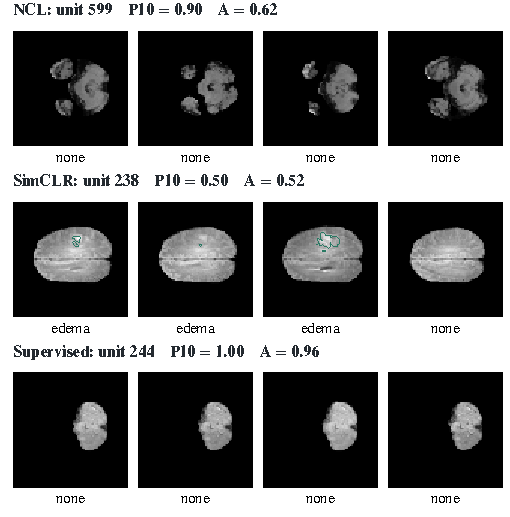
\includegraphics[width=\columnwidth]{figures/feature_examples.pdf}
\caption{Top activating inputs from archived SAEs (encoder and SAE seed 10). Each row selects the unit with the largest cumulative positive training count, breaking ties by feature index, then shows its four highest positive validation inputs. $P10$ uses all ten top inputs; $A$ uses training oriented AUROC. Labels denote dominant regions; green contours are annotations, not activations. Patients may repeat. These examples are not a matched comparison or expert validation.}
\label{fig:featureexamples}
\end{figure}

Figure~\ref{fig:featureexamples} shows the slices that most strongly activate features selected by training activity. Some galleries have high purity because their slices show no tumour. The galleries alone cannot identify a medical concept.

\subsection{The budget curve exposes gallery selection dependence}
Figure~\ref{fig:budgetaudit} shows how the gap changes across budgets. With features eligible on validation, the NCL minus SimCLR gap is $-8.19$ points at $J=8$, $-3.06$ at 32, $-0.10$ at 64 and $+1.04$ at 80. The mean crosses zero near $J=70$, but the patient envelopes include zero at $J=32,64,80$. They span $[-2.76,3.16]$ at 64 and $[-2.40,4.28]$ at 80. At $J=8$, the envelope is $[-12.50,-1.25]$. At $J=64$, only 2.4\% of draws can score every selected feature in every dictionary. We keep the other draws by using bounds. Panel A shows each dictionary up to its own endpoint, which can differ across dictionaries.

With selection based on training alone, NCL purity at $J=64$ is 82.80\% among scorable features. Coverage is 94.79\%. The bounds for all 64 features (78.54 to 83.75\%) include SimCLR's 83.13\%. NCL coverage drops to 90.97\% at $J=80$. Supervised coverage is 87.50\% at $J=64$. The bounds keep every selected feature in the comparison.

\subsection{Random subsets and the supervised reference}
At $J=64$, usage ranked purity minus the random subset mean is $-0.98$ points for NCL, $+3.25$ for SimCLR and $+7.14$ for the supervised reference. These conditional selection references do not establish patient level significance; per dictionary quantiles remain in the artifact.

The supervised reference has all eligible purity 79.79\%, below NCL, but $J=8$ purity 99.31\%, above NCL (79.86\%) and SimCLR (88.06\%). Its direct tumour presence objective and different augmentations make this an expected reference, not evidence across architectures or datasets.

\subsection{Aggregate prediction is a different comparison}
Macro F1 measures tumour presence prediction. SimCLR leads on raw embeddings (87.88\% versus 84.80\%) and full SAE codes (87.51\% versus 83.59\%). With 64 selected features, NCL leads (83.45\% versus 77.12\%) at nearly equal purity.

These probes measure what features predict together. The AUROC analysis tests each feature separately. Both analyses use slice labels and leave clinical benefit untested.

\section{Discussion and Limits}
\paragraph{What the audits add.}
The budget curves show how purity changes with the number of displayed features. Random subsets show how much the ranking rule matters. Coverage and bounds show how missing scores could affect the comparison. The shuffle reference shows what remains after accounting for tumour area and slice position. The feature correlations describe a separate aspect of prediction, with the shared target structure limiting how we can interpret them.

\paragraph{Reading the audit as a model comparison.}
Using all eligible features gives NCL a 4.11 point lead in raw purity, with different numbers of features for each method. Holding the budget at 64 brings the mean gap close to zero. The stratified shuffle asks whether the top slices share labels more often than we would expect from tumour area and position alone. Under patient resampling, that gap also includes zero. Together, these results give little support for a stable purity lead and leave open whether the methods perform equally. 

\begingroup\interlinepenalty=10000
Prediction depends on the representation: SimCLR leads on raw embeddings and full SAE codes, while NCL leads on the 64 selected features. A gallery alone is therefore a poor basis for choosing a model.
\par\endgroup

\begingroup\widowpenalties 3 10000 10000 0\relax
\paragraph{Deployment oriented use.}
We recommend naming the feature population and giving its size for each model. Show purity over several matched budgets. Report coverage and bounds for features without enough evaluation examples. Include a random subset reference from the same dictionary, and show raw purity alongside excess over a shuffle that preserves annotation context. For prediction, specify whether the probe uses raw embeddings, full codes or selected codes. These checks help readers assess a feature gallery before relying on it. Clinical use still requires validation.
\par\endgroup

\paragraph{Evidence and optimization.}
The study uses FLAIR, ViT Tiny, three encoder seeds and 37 patients from the original validation cohort. Fitting several SAEs to one encoder does not add independent encoders. The 50 epoch budget gives both methods the same number of epochs, but NCL's validation loss remains noisy and convergence is uncertain. Model selection can affect later evaluation \cite{cawley2010selection}, and small imaging cohorts bring substantial uncertainty \cite{varoquaux2018crossvalidation}. Earlier models already used the registered test patients, so this study provides no fresh patient evaluation. The supervised reference also differs in objective and augmentations, which prevents us from isolating the effect of the objective.

\paragraph{Meaning of the target.}
Purity measures how often the top slices share a label. Tumour area may be clinically relevant, and the stratified shuffle tests what purity remains after accounting for it. Other ways to group the slices could give different results. AUROC for one feature cannot capture effects that depend on combinations of features. Establishing a medical concept, locating it in an image or showing that experts agree would require separate evidence.

\paragraph{Reproducibility.}
The archive includes settings, hashes for inputs and model states, 27 feature tables, shuffle definitions, bootstrap outputs and nine supervised SAE states. The original encoder weights are unavailable, but the saved vectors let us repeat the audits. A separate run preserved six encoders and 18 SAEs and verified inference. The paper's original results use the historical vectors.

\section{Conclusion}
Average purity rankings change with the feature budget, while the uncertainty envelopes for larger budgets include zero. Accounting for tumour area and slice position also changes the purity comparison. Purity and tumour presence AUROC share information about the labels, which limits what their correlation can tell us. Reporting the feature selection rule, coverage, shuffle reference and prediction inputs makes these comparisons easier to interpret. Clinical validity still requires further evaluation.

OpenAI Codex assisted with experiment and analysis code, figures and writing and revising the manuscript. The human author takes responsibility for the scientific claims, references, code and all submitted content. Codex did not serve as an author or a source of scientific evidence.

\bibliography{references}

\appendix
\setlength{\parskip}{0pt}
\section{Reading and Reusing the Audit Artifact}
\paragraph{Identify the experimental unit.}
Each dictionary comes from one encoder seed and one SAE seed. We average the three SAE fits for each encoder, then summarize the three encoder averages. The nine dictionaries share three encoders. Resampling patients measures variation in the cohort for these fitted models.

\paragraph{Keep selection and scoring separate.}
For a matched budget, record the requested number of features, their IDs and the ranking rule. One analysis selects from features eligible on validation. The other fixes eligibility and rank using training activity alone. If a selected feature has fewer than ten positive evaluation slices, keep its place and report how many features can be scored. Read the average for scorable features alongside the bounds for the full budget.

\paragraph{Distinguish the two reference distributions.}
Use random subsets to ask whether ranking by activity selects features with higher purity than other features in the same dictionary. Use stratified label shuffles to ask whether purity exceeds what we expect given tumour area and slice position. A separate zero area group preserves absence, so a feature can detect absence and still show little excess. Report both raw purity and excess to show what each comparison captures.

\paragraph{Connect a feature to prediction.}
Univariate AUROC tests one activation with training fixed orientation; joint probes can exploit combinations. Neither establishes spatial or expert validity. Near zero excess correlations do not imply that codes lack predictive information.

\paragraph{Separate analysis reuse from image inference.}
Saved vectors, dictionary states and feature selection records let us repeat the audits. To run inference on images, we also need the encoder and its preprocessing. The weights from the preservation run belong to separate models. Keep each embedding linked to the model that produced it.

\paragraph{A numerical coverage example.}
Suppose a frozen list requests 64 features, but only 60 have enough positive evaluation activations to score. This is an illustration, not an additional experimental result. If those 60 features have mean purity 0.80, their observed purity sum is 48. The four missing scores can each lie between zero and one. The mean over all 64 requested features is therefore bounded by $48/64=0.75$ and $52/64=0.8125$, while coverage is $60/64=93.75\%$. Reporting 0.80 alone would conceal this distinction. If another method scored 0.79 with complete coverage, the conditional means would favor the first method, but the bounds would not identify a winner. The reported training only 64 feature comparison has this same interpretive issue, although its actual dictionary specific bounds are computed before aggregation.

\paragraph{What a context conditioned null detects.}
A feature selecting only slices without annotated tumour can obtain perfect raw purity. Because zero tumour area forms its own stratum, shuffling within that cell preserves the absence label and also produces perfect reference purity. Zero excess is then the intended answer: the feature has not selected labels more narrowly than that context predicts. In a cell containing several region labels, a feature consistently selecting one region can instead exceed the within cell reference. This contrast explains why raw purity and stratified excess need not agree. It also shows why excess should not replace raw purity when tumour presence itself is the prediction target.

\section{Additional Related Work Context}\label{app:relatedcontext}
\paragraph{Sparse representation choices.}
Sparse coding connects learned visual directions to image statistics \cite{olshausen1996sparse}; k sparse autoencoders impose explicit activation budgets \cite{makhzani2013ksparse}. Language model SAEs demonstrate dictionary based feature analysis \cite{cunningham2023sparse}. These precedents motivate separating reconstruction, activation sparsity and the label selectivity of the surviving units rather than interpreting a small feature population as sufficient evidence of semantic quality.

\paragraph{Other visual learning objectives.}
Momentum contrast uses an evolving encoder for comparison targets \cite{he2020moco}. BYOL and SimSiam learn paired representations without explicit negative pairs \cite{grill2020byol,chen2021simsiam}, while SwAV uses cluster assignments \cite{caron2020swav}. DINO and DINOv2 use self distillation \cite{caron2021dino,oquab2023dinov2}; Barlow Twins and VICReg explicitly address redundancy or variance \cite{zbontar2021barlow,bardes2022vicreg}. Partial collapse also occurs in noncontrastive learning \cite{li2022collapse}. These are relevant alternatives, not additional baselines evaluated in our encoder comparison.

\paragraph{Encoder side remedies.}
Medical contrastive learning has considered whitening to address dimensional collapse \cite{hassanpour2024collapse}. SACReg targets spectral collapse and is applied to JEPA as $\lambda$ JEPA \cite{demirel2026sacreg}. Our descriptive geometry controls do not evaluate these remedies or identify a causal effect of geometry; their inclusion here locates an experimental gap rather than resolving it.

\paragraph{Attribution and validity.}
LIME, Integrated Gradients and SHAP explain predictions through local approximations or attribution rules \cite{ribeiro2016lime,sundararajan2017axiomatic,lundberg2017shap}. Sanity checks and input invariance analyses show why visual appeal alone cannot validate an explanation \cite{adebayo2018sanity,kindermans2017reliability}. Interpretable model arguments and work on monosemanticity and robustness further distinguish prediction, explanation and robustness outcomes \cite{rudin2019interpretable,zhang2025beyond}. Slice label concentration is narrower than these targets.

\paragraph{Predictive measurement.}
ROC analysis evaluates score ranking \cite{fawcett2006roc}; precision recall analysis emphasizes performance on the positive class under imbalance \cite{saito2015precision}. These perspectives complement the reported class averaged F1 comparison but cannot establish that a feature expresses a clinically meaningful concept.

\section{Interpreting the Audit Outputs}
This guide explains how to read the existing audit outputs together. It introduces no additional experiments, model fits or numerical results.

\paragraph{When a gallery comparison changes with budget.}
Check that both methods contribute the same number of features and retain the ranking rule across budgets. All eligible averages describe each dictionary's population; matched budgets describe selected subsets. These can disagree without either calculation being incorrect. Report the common comparison domain rather than selecting the most favorable budget.

\paragraph{When conditional purity exceeds the bounded comparison.}
The conditional mean covers only features we can score. Coverage gives their share of the requested list. The full budget bounds show how much the missing scores could change the average. If a competing score falls inside those bounds, the conditional means alone cannot rank the methods. Showing more examples does not score the missing features.

\paragraph{When excess purity is small.}
Inspect what the shuffle reference preserves before treating a small excess as feature failure. The stratified reference retains coarse tumour area and axial position, including a separate tumour absence cell. A unit responding to one of those properties may remain useful for prediction while showing little concentration beyond that reference. Present raw purity and excess together so the reader can distinguish label concentration from concentration beyond the specified context.

\paragraph{When predictive comparisons disagree.}
Identify whether the probe uses raw embeddings, the full SAE code or a selected code. A change in the prediction representation changes which combinations of information are available to the classifier. A joint probe can exploit complementary activations even when individual units have modest associations with the target. Conversely, a concentrated top example list does not show that the associated activation is sufficient for accurate prediction across the cohort.

\paragraph{When a resampling envelope crosses zero.}
A mean crossing shows where the average changes sign. Check the envelope before claiming that the ranking would change across patients. The envelope holds models and selected features fixed and excludes variation from retraining or redesigning the analysis. It describes one budget at a time.

\paragraph{What to retain for subsequent evaluation.}
Retain the manifest, model identity, selected IDs, support and ranking rules, probe representation and shuffle strata. Record how intervals treat missing support. Freeze these choices before inspecting new patient outcomes.

\end{document}
